\documentclass{article}
\usepackage[utf8]{inputenc}
\usepackage[spanish]{babel}
\usepackage{listings}
\usepackage{graphicx}
\graphicspath{ {images/} }
\usepackage{cite}

\begin{document}

\begin{titlepage}
    \begin{center}
        \vspace*{1cm}
            
        \Huge
        \textbf{Proyecto Parcial I}
            
        \vspace{0.5cm}
        \LARGE
        Informatica II
            
        \vspace{1.5cm}
            
        \textbf{Pedro Luis López Santiago}
        
        \textbf{Alejandro Lopera Gutierrez}
        
        \textbf{Juan David Jimenez Osorio}        
        
        \vfill
            
        \vspace{0.8cm}
            
        \Large
        Departamento de Ingeniería Electrónica y Telecomunicaciones\\
        Universidad de Antioquia\\
        Medellín\\
        Marzo de 2021
            
    \end{center}
\end{titlepage}

\tableofcontents
\newpage
\section{Introduccion}\label{intro}
Mediante el uso de herramientas nombradas y utilizadas en las clases de informatica II, de la Universidad de Antioquia, se llevara a cabo una serie de ejercicios y mecanismos utilizados para ejercer o darle forma a un proyecto, el cual será un panel de 8x8 leds, totalmente funcionable, el cual pueda reflejar cierta secuencia de iluminacion reflejando ante los ojos del receptor una forma conocida, ya sea un numero o una letra.
Se tendran en cuenta una serie de criterios y normas establecidas por el docente a cargo de la materia, como trabajar desde tinkercad, utilizando cierta cantidad de pines y tambien utilizando un integrado en especifico.
Tiene un alto nivel de logica el proyecto a trabajar y se necesitara de un desenvolvimiento en equipo donde todos los miembros de este trabajen de forma armonica para que puedan darle forma final con exito.

\section{Analisis del problema} \label{contenido}
Como problema a resolver, piden hacer un panel de leds 8x8 totalmente funcional, que refleje una secuencia especifica solicitada por el usuario.
Se debe trabajar bajo ciertos parametros establecidos.

-Trabajar con arduino 1

-No usar más de 7 pines

-Usar el integrado 74HC595

-Se debe incluir apuntadores y arreglos en el codigo utilizado

-Se necesita hacer un esquema

El proyecto se realiza en un equipo integrado por 3 estudiantes que analizaran, discutiran y trabajaran de manera armonica para completar la tarea con exito.


\subsection{Manual de uso del usuario}


En el codigo se declaran primero los pibes a utilizar que serian 
el pin 2, 3 y 4 y se define un parametro tiempo que nos ayudara
a ejecutar las lineas

La funcion ledWrite nos permite escribir una secuencia binaria que
se mostrara linea a linea.
En las funciones void se ejecutan los esquemas de las formas que 
queremos.
son 8 digitalwrite, esto porque la matriz tiene 8 filas
y tiene tambien 1 byte cada digital write.
La secuencia se imprime de abajo para arriba, es decir.
La ultima fila en el codigo es la primera en los leds.

Luego en el void loop están los if, que evaluan que caracter ingresa el 
usuario y depende a lo que ingrese lo imprime en la matriz.*/

\subsection{código en el documento}
//Funcionamiento y desarrollo de las funciones que se encargaran de mostrar un patron de letras y numeros en los leds del circuito 


int pinData  = 2;

int pinLatch = 3;

int pinClock = 4;

#define TIEMPO 15


void ledWrite(int Led){
   
   shiftOut(pinData, pinClock, LSBFIRST, Led);
   
   digitalWrite(pinLatch, HIGH);
   
   digitalWrite(pinLatch, LOW);
}

void Num9(){
     
   ledWrite(B00000111); delay(TIEMPO);
   
   ledWrite(B00000111); delay(TIEMPO);
   
   ledWrite(B00000111); delay(TIEMPO);
   
   ledWrite(B11111111); delay(TIEMPO);
   
   ledWrite(B11000111); delay(TIEMPO);
   
   ledWrite(B11000111); delay(TIEMPO);
   
   ledWrite(B11111111); delay(TIEMPO);
   
   ledWrite(B11111111); delay(TIEMPO);
  
  delay(500000000000000000);}
  
void Num8(){
     
   ledWrite(B11111111); delay(TIEMPO);
   
   ledWrite(B11100111); delay(TIEMPO);
   
   ledWrite(B11000011); delay(TIEMPO);
   
   ledWrite(B11111111); delay(TIEMPO);
   
   ledWrite(B11111111); delay(TIEMPO);
   
   ledWrite(B11000011); delay(TIEMPO);
   
   ledWrite(B11100111); delay(TIEMPO);
   
   ledWrite(B11111111); delay(TIEMPO);
  
  delay(500000000000000000);}
  
void Num7(){

   ledWrite(B11100000); delay(TIEMPO);

   ledWrite(B01110000); delay(TIEMPO);

   ledWrite(B00111000); delay(TIEMPO);

   ledWrite(B00011100); delay(TIEMPO);

   ledWrite(B00001110); delay(TIEMPO);

   ledWrite(B00000111); delay(TIEMPO);

   ledWrite(B11111111); delay(TIEMPO);

   ledWrite(B11111111); delay(TIEMPO);

  delay(500000000000000000);}
  
void Num6(){
   
   ledWrite(B11111111); delay(TIEMPO);
   
   ledWrite(B11111111); delay(TIEMPO);
   
   ledWrite(B11100011); delay(TIEMPO);
   
   ledWrite(B11111111); delay(TIEMPO);
   
   ledWrite(B11111111); delay(TIEMPO);
   
   ledWrite(B11000000); delay(TIEMPO);
   
   ledWrite(B11111111); delay(TIEMPO);
   
   ledWrite(B11111111); delay(TIEMPO);
  
  delay(500000000000000000);}
  
void Num5(){
     
     ledWrite(B11111111); delay(TIEMPO);
   
   ledWrite(B11111111); delay(TIEMPO);
   
   ledWrite(B00000111); delay(TIEMPO);
   
   ledWrite(B11111111); delay(TIEMPO);
   
   ledWrite(B11111111); delay(TIEMPO);
   
   ledWrite(B11100000); delay(TIEMPO);
   
   ledWrite(B11111111); delay(TIEMPO);
   
   ledWrite(B11111111); delay(TIEMPO);
  
  delay(500000000000000000);}

void Num4(){
     
   ledWrite(B00000111); delay(TIEMPO);
   
   ledWrite(B00000111); delay(TIEMPO);
   
   ledWrite(B00000111); delay(TIEMPO);
   
   ledWrite(B11111111); delay(TIEMPO);
   
   ledWrite(B11111111); delay(TIEMPO);
   
   ledWrite(B01100011); delay(TIEMPO);
   
   ledWrite(B00110011); delay(TIEMPO);
   
   ledWrite(B00011111); delay(TIEMPO);
  
  delay(500000000000000000);}

void Num3(){
      
   ledWrite(B11111111); delay(TIEMPO);
   
   ledWrite(B11111111); delay(TIEMPO);
   
   ledWrite(B00000011); delay(TIEMPO);
   
   ledWrite(B11111111); delay(TIEMPO);
   
   ledWrite(B11111111); delay(TIEMPO);
   
   ledWrite(B00000011); delay(TIEMPO);
   
   ledWrite(B11111111); delay(TIEMPO);
   
   ledWrite(B11111111); delay(TIEMPO);
  
  delay(500000000000000000);}

void Num2(){
     
   ledWrite(B11111111); delay(TIEMPO);
   
   ledWrite(B11111111); delay(TIEMPO);
   
   ledWrite(B11100000); delay(TIEMPO);
   
   ledWrite(B11111111); delay(TIEMPO);
   
   ledWrite(B11111111); delay(TIEMPO);
   
   ledWrite(B00000111); delay(TIEMPO);
   
   ledWrite(B11111111); delay(TIEMPO);
   
   ledWrite(B11111111); delay(TIEMPO);
  
  delay(500000000000000000);}

void Num1(){ 
   
   ledWrite(B00000111); delay(TIEMPO);
   
   ledWrite(B00000111); delay(TIEMPO);
   
   ledWrite(B00000111); delay(TIEMPO);
   
   ledWrite(B00000111); delay(TIEMPO);
   
   ledWrite(B01110111); delay(TIEMPO);
   
   ledWrite(B00111111); delay(TIEMPO);
   
   ledWrite(B00011111); delay(TIEMPO);
   
   ledWrite(B00001111); delay(TIEMPO);
  
  delay(500000000000000000);}

void Num0(){
   
   ledWrite(B11111111); delay(TIEMPO);
   
   ledWrite(B11100111); delay(TIEMPO);
   
   ledWrite(B11000011); delay(TIEMPO);
   
   ledWrite(B11000011); delay(TIEMPO);
   
   ledWrite(B11000011); delay(TIEMPO);
   
   ledWrite(B11000011); delay(TIEMPO);
   
   ledWrite(B11100111); delay(TIEMPO);
   
   ledWrite(B11111111); delay(TIEMPO);
  
  delay(500000000000000000);}
  
void LetraA (){
   
   ledWrite(B11000011); delay(TIEMPO);
   
   ledWrite(B11000011); delay(TIEMPO);
   
   ledWrite(B11111111); delay(TIEMPO);
   
   ledWrite(B11111111); delay(TIEMPO);
   
   ledWrite(B11100111); delay(TIEMPO);
   
   ledWrite(B01100110); delay(TIEMPO);
   
   ledWrite(B00111100); delay(TIEMPO);
   
   ledWrite(B00011000); delay(TIEMPO);
  
  delay(500000000000000000);}

void LetraB(){
     
   ledWrite(B11111110); delay(TIEMPO);
   
   ledWrite(B11111111); delay(TIEMPO);
   
   ledWrite(B11000011); delay(TIEMPO);
   
   ledWrite(B11111110); delay(TIEMPO);
   
   ledWrite(B11111110); delay(TIEMPO);
   
   ledWrite(B11000011); delay(TIEMPO);
   
   ledWrite(B11111111); delay(TIEMPO);
   
   ledWrite(B11111110); delay(TIEMPO);
  
  delay(500000000000000000);}

void LetraC(){
   
   ledWrite(B11111111); delay(TIEMPO);
   
   ledWrite(B11111111); delay(TIEMPO);
   
   ledWrite(B11100000); delay(TIEMPO);
   
   ledWrite(B11100000); delay(TIEMPO);
   
   ledWrite(B11100000); delay(TIEMPO);
   
   ledWrite(B11100000); delay(TIEMPO);
   
   ledWrite(B11111111); delay(TIEMPO);
   
   ledWrite(B11111111); delay(TIEMPO);
  
  delay(500000000000000000);}

void LetraD(){
   
   ledWrite(B11111110); delay(TIEMPO);
   
   ledWrite(B11111111); delay(TIEMPO);
   
   ledWrite(B11100011); delay(TIEMPO);
   
   ledWrite(B11100011); delay(TIEMPO);
   
   ledWrite(B11100011); delay(TIEMPO);
   
   ledWrite(B11100011); delay(TIEMPO);
   
   ledWrite(B11111111); delay(TIEMPO);
   
   ledWrite(B11111110); delay(TIEMPO);
   
   delay(500000000000000000);}

void LetraE(){
   
   ledWrite(B11111111); delay(TIEMPO);
   
   ledWrite(B11111111); delay(TIEMPO);
   
   ledWrite(B11100000); delay(TIEMPO);
   
   ledWrite(B11111111); delay(TIEMPO);
   
   ledWrite(B11111111); delay(TIEMPO);
   
   ledWrite(B11100000); delay(TIEMPO);
   
   ledWrite(B11111111); delay(TIEMPO);
   
   ledWrite(B11111111); delay(TIEMPO);
   
   delay(500000000000000000);}

void LetraF(){
   
   ledWrite(B11100000); delay(TIEMPO);
   
   ledWrite(B11100000); delay(TIEMPO);
   
   ledWrite(B11100000); delay(TIEMPO);
   
   ledWrite(B11111111); delay(TIEMPO);
   
   ledWrite(B11111111); delay(TIEMPO);
   
   ledWrite(B11100000); delay(TIEMPO);
   
   ledWrite(B11111111); delay(TIEMPO);
   
   ledWrite(B11111111); delay(TIEMPO);
   
   delay(500000000000000000);}

void LetraG(){
   
   ledWrite(B11111111); delay(TIEMPO);
   
   ledWrite(B11111111); delay(TIEMPO);
   
   ledWrite(B11000011); delay(TIEMPO);
   
   ledWrite(B11001111); delay(TIEMPO);
   
   ledWrite(B11001111); delay(TIEMPO);
   
   ledWrite(B11000000); delay(TIEMPO);
   
   ledWrite(B11111111); delay(TIEMPO);
   
   ledWrite(B11111111); delay(TIEMPO);
  
  delay(500000000000000000);}

void LetraH(){
   
   ledWrite(B11100111); delay(TIEMPO);
   
   ledWrite(B11100111); delay(TIEMPO);
   
   ledWrite(B11100011); delay(TIEMPO);
   
   ledWrite(B11111111); delay(TIEMPO);
   
   ledWrite(B11111111); delay(TIEMPO);
   
   ledWrite(B11100111); delay(TIEMPO);
   
   ledWrite(B11100111); delay(TIEMPO);
   
   ledWrite(B11100111); delay(TIEMPO);
   
   delay(500000000000000000);}

void LetraI(){
   
   ledWrite(B11111111); delay(TIEMPO);
   
   ledWrite(B11111111); delay(TIEMPO);
   
   ledWrite(B00011000); delay(TIEMPO);
   
   ledWrite(B00011000); delay(TIEMPO);
   
   ledWrite(B00011000); delay(TIEMPO);
   
   ledWrite(B00011000); delay(TIEMPO);
   
   ledWrite(B11111111); delay(TIEMPO);
   
   ledWrite(B11111111); delay(TIEMPO);
   
   delay(500000000000000000);}

void LetraJ(){
   
   ledWrite(B11111111); delay(TIEMPO);
   
   ledWrite(B11111111); delay(TIEMPO);
   
   ledWrite(B11100011); delay(TIEMPO);
   
   ledWrite(B00000111); delay(TIEMPO);
   
   ledWrite(B00000111); delay(TIEMPO);
   
   ledWrite(B01000111); delay(TIEMPO);
   
   ledWrite(B11111111); delay(TIEMPO);
   
   ledWrite(B11111111); delay(TIEMPO);
   
   delay(500000000000000000);}

void LetraK(){
   
   ledWrite(B11100010); delay(TIEMPO);
   
   ledWrite(B11100110); delay(TIEMPO);
   
   ledWrite(B11101100); delay(TIEMPO);
   
   ledWrite(B11110000); delay(TIEMPO);
   
   ledWrite(B11110000); delay(TIEMPO);
   
   ledWrite(B11101100); delay(TIEMPO);
   
   ledWrite(B11100110); delay(TIEMPO);
   
   ledWrite(B11100010); delay(TIEMPO);
   
   delay(500000000000000000);}

void LetraL(){
   
   ledWrite(B11111111); delay(TIEMPO);
   
   ledWrite(B11111111); delay(TIEMPO);
   
   ledWrite(B11100000); delay(TIEMPO);
   
   ledWrite(B11100000); delay(TIEMPO);
   
   ledWrite(B11100000); delay(TIEMPO);
   
   ledWrite(B11100000); delay(TIEMPO);
   
   ledWrite(B11100000); delay(TIEMPO);
   
   
   ledWrite(B11100000); delay(TIEMPO);
   
   delay(500000000000000000);}

void LetraM(){
   
   ledWrite(B11000011); delay(TIEMPO);
   
   ledWrite(B11000011); delay(TIEMPO);
   
   ledWrite(B11000011); delay(TIEMPO);
   
   ledWrite(B11011011); delay(TIEMPO);
   
   ledWrite(B11011011); delay(TIEMPO);
   
   ledWrite(B11111111); delay(TIEMPO);
   
   ledWrite(B11100111); delay(TIEMPO);
   
   ledWrite(B11000011); delay(TIEMPO);
   
   delay(500000000000000000);}

void LetraN(){
   
   ledWrite(B11000011); delay(TIEMPO);
   
   ledWrite(B11000011); delay(TIEMPO);
   
   ledWrite(B11000111); delay(TIEMPO);
   
   ledWrite(B11001111); delay(TIEMPO);
   
   ledWrite(B11011011); delay(TIEMPO);
   
   ledWrite(B11110011); delay(TIEMPO);
   
   ledWrite(B11100011); delay(TIEMPO);
   
   ledWrite(B11000011); delay(TIEMPO);
  
  delay(500000000000000000);}

void LetraO(){
   
   ledWrite(B01111110); delay(TIEMPO);
   
   ledWrite(B01111110); delay(TIEMPO);
   
   ledWrite(B11000011); delay(TIEMPO);
   
   ledWrite(B11000011); delay(TIEMPO);
   
   ledWrite(B11000011); delay(TIEMPO);
   
   ledWrite(B11000011); delay(TIEMPO);
   
   ledWrite(B01111110); delay(TIEMPO);
   
   ledWrite(B01111110); delay(TIEMPO);
  
  delay(500000000000000000);}

void LetraP(){

   ledWrite(B11000000); delay(TIEMPO);

   ledWrite(B11000000); delay(TIEMPO);

   ledWrite(B11000000); delay(TIEMPO);

   ledWrite(B11110000); delay(TIEMPO);

   ledWrite(B11111111); delay(TIEMPO);

   ledWrite(B11000011); delay(TIEMPO);

   ledWrite(B11000011); delay(TIEMPO);

   ledWrite(B11111111); delay(TIEMPO);

  delay(500000000000000000);}

void LetraQ(){

   ledWrite(B00000001); delay(TIEMPO);

   ledWrite(B11111110); delay(TIEMPO);

   ledWrite(B11000111); delay(TIEMPO);

   ledWrite(B11001011); delay(TIEMPO);

   ledWrite(B11000011); delay(TIEMPO);

   ledWrite(B11000011); delay(TIEMPO);

   ledWrite(B11000011); delay(TIEMPO);

   ledWrite(B11111111); delay(TIEMPO);

   delay(500000000000000000);}

void LetraR(){

   ledWrite(B10001100); delay(TIEMPO);

   ledWrite(B10011000); delay(TIEMPO);

   ledWrite(B10110000); delay(TIEMPO);

   ledWrite(B11100000); delay(TIEMPO);

   ledWrite(B11111000); delay(TIEMPO);

   ledWrite(B10000100); delay(TIEMPO);

   ledWrite(B10000100); delay(TIEMPO);

   ledWrite(B11111000); delay(TIEMPO);

   delay(500000000000000000);}

void LetraS(){

   ledWrite(B11111110); delay(TIEMPO);

   ledWrite(B11111111); delay(TIEMPO);

   ledWrite(B00000011); delay(TIEMPO);

   ledWrite(B00000011); delay(TIEMPO);

   ledWrite(B01111110); delay(TIEMPO);

   ledWrite(B11000000); delay(TIEMPO);

   ledWrite(B11111111); delay(TIEMPO);

   ledWrite(B01111111); delay(TIEMPO);

  delay(500000000000000000);}

void LetraT(){

   ledWrite(B00011000); delay(TIEMPO);

   ledWrite(B00011000); delay(TIEMPO);

   ledWrite(B00011000); delay(TIEMPO);

   ledWrite(B00011000); delay(TIEMPO);

   ledWrite(B00011000); delay(TIEMPO);

   ledWrite(B00011000); delay(TIEMPO);

   ledWrite(B11111111); delay(TIEMPO);

   ledWrite(B11111111); delay(TIEMPO);

  delay(500000000000000000);}

void LetraU(){

   ledWrite(B11111111); delay(TIEMPO);

   ledWrite(B11111111); delay(TIEMPO);

   ledWrite(B11000011); delay(TIEMPO);

   ledWrite(B11000011); delay(TIEMPO);

   ledWrite(B11000011); delay(TIEMPO);

   ledWrite(B11000011); delay(TIEMPO);

   ledWrite(B11000011); delay(TIEMPO);

   ledWrite(B11000011); delay(TIEMPO);

  delay(500000000000000000);}

void LetraV(){

   ledWrite(B00011000); delay(TIEMPO);

   ledWrite(B00111100); delay(TIEMPO);

   ledWrite(B01100110); delay(TIEMPO);

   ledWrite(B11000011); delay(TIEMPO);

   ledWrite(B11000011); delay(TIEMPO);

   ledWrite(B11000011); delay(TIEMPO);

   ledWrite(B11000011); delay(TIEMPO);

   ledWrite(B11000011); delay(TIEMPO);

  delay(500000000000000000);}

void LetraW(){

   ledWrite(B11111111); delay(TIEMPO);

   ledWrite(B11111111); delay(TIEMPO);

   ledWrite(B11011011); delay(TIEMPO);

   ledWrite(B11011011); delay(TIEMPO);

   ledWrite(B11011011); delay(TIEMPO);

   ledWrite(B11000011); delay(TIEMPO);

   ledWrite(B11000011); delay(TIEMPO);

   ledWrite(B11000011); delay(TIEMPO);

  delay(500000000000000000);}

void LetraX(){

   ledWrite(B11000011); delay(TIEMPO);

   ledWrite(B01100110); delay(TIEMPO);

   ledWrite(B00111100); delay(TIEMPO);

   ledWrite(B00011000); delay(TIEMPO);


   ledWrite(B00111100); delay(TIEMPO);

   ledWrite(B01100110); delay(TIEMPO);

   ledWrite(B11000011); delay(TIEMPO);

   ledWrite(B00000000); delay(TIEMPO);

  delay(500000000000000000);}

void LetraY(){

   ledWrite(B00011000); delay(TIEMPO);

   ledWrite(B00011000); delay(TIEMPO);

   ledWrite(B00011000); delay(TIEMPO);

   ledWrite(B00011000); delay(TIEMPO);

   ledWrite(B00011000); delay(TIEMPO);

   ledWrite(B01100100); delay(TIEMPO);

   ledWrite(B01100110); delay(TIEMPO);

   ledWrite(B11000011); delay(TIEMPO);

  delay(500000000000000000);}

void LetraZ(){

   ledWrite(B00000000); delay(TIEMPO);

   ledWrite(B11111111); delay(TIEMPO);

   ledWrite(B11000000); delay(TIEMPO);

   ledWrite(B00110000); delay(TIEMPO);

   ledWrite(B00001100); delay(TIEMPO);

   ledWrite(B00000011); delay(TIEMPO);

   ledWrite(B11111111); delay(TIEMPO);

   ledWrite(B00000000); delay(TIEMPO);

  delay(500000000000000000);}

void verificacion(){
  

   ledWrite(B11111111); delay(TIEMPO);

   ledWrite(B11111111); delay(TIEMPO);

   ledWrite(B11111111); delay(TIEMPO);

   ledWrite(B11111111); delay(TIEMPO);

   ledWrite(B11111111); delay(TIEMPO);

   ledWrite(B11111111); delay(TIEMPO);

   ledWrite(B11111111); delay(TIEMPO);

   ledWrite(B11111111); delay(TIEMPO);

  delay(500000000000000000);}

char let='+';

void setup(){

  Serial.begin(9600);

  pinMode(pinData, OUTPUT);

  pinMode(pinLatch, OUTPUT);

  pinMode(pinClock, OUTPUT);

  Serial.println("Ingrese V para funcion verificacion "); 

  Serial.println("Ingrese cualquier caracter en minuscula para 
  verlo en el circuito");
    
 Serial.println("Ingrese un numero del 0 al 9 para verlo en el circuito"); 

  
}
  if (let == 'a') {
    LetraA();}
  
  if (let == 'b'){
    LetraB();}
  
  if (let == 'c') {
    LetraC();}
  
  if (let == 'd') {
    LetraD();}
  
  if (let == 'e') {
    LetraE();}
  
  if (let == 'f') {
    LetraF();}

  if (let == 'g') {
    LetraG();}

  if (let == 'h') {
    LetraH();}

  if (let == 'i') {
    LetraI();}

  if (let == 'j') {
    LetraJ();}

  if (let == 'k') {
    LetraK();}

  if (let == 'l') {
    LetraL();}

  if (let == 'm') {
    LetraM();}

  if (let == 'n') {
    LetraN();}

  if (let == 'o') {
    LetraO();}

  if (let == 'p') {
    LetraP();}

  if (let == 'q') {
    LetraQ();}

   if (let == 'r') {
    LetraR();}

  if (let == 's') {
    LetraS();}

  if (let == 't') {
    LetraT();}

  if (let == 'u') {
    LetraU();}

  if (let == 'v') {
    LetraV();}

  if (let == 'w') {
    LetraW();}

  if (let == 'x') {
    LetraX();}

  if (let == 'y') {
    LetraY();}

  if (let == 'z') {
    LetraZ();}

  if (let=='verificacion'){
    verificacion();}


  if (let == '1'){
    Num1();}
  
  if (let == '2'){
    Num2();}
  
  if (let == '3'){
    Num3();}
  
  if (let == '4'){
    Num4();}
  
  if (let == '5'){
    Num5();}
  
  if (let == '6'){
    Num6();}
  
  if (let == '7'){
    Num7();}
  
  if (let == '8'){
    Num8();}
  
  if (let == '9'){
    Num9();}
  
  if (let == '0'){
    Num0();}
  
\subsection{Problemas Al Realizar El Circuito }
Al momento en que comenzamos a realizar el circuito surguieron varias preguntas del como iria toda la conexion para poder darle un buen funicionamiento a todos los leds y los demas elementos implementados para el dasarrollo del problema, para la solucion de estas preguntas nos guiamos de la conexion de una matriz de leds de 8x8 ya creada, pero implementando las condiciones puestas por el profesor. al terminar de hacer la elaboracion del circuito, lo empezamos a probar y nos dimos cuenta de que al momento de imprimir algunas letras o numeros, quedaban algunos leds apagados, por lo cual, realizamos una revision de todas las resistencias y de los leds y nos pudimos dar cuenta de que habian problemas en varias conexiones. Le pudimos dar solucion a este problema y ya al momento de ver su funcionamiento, todo iba correcto y imprimia las letras y numeros de nanera adecuada. 

\subsection{Problemas Al Realizar El codigo}
Una vez esquematizado el circuito y realizado las conexiones, abrimos paso a ejemplificar y planificar los medios y estrategias que se ejecutarian a la hora de realizar el codigo, como primera medida se tomo como referencia base un codigo hayado en internet. Posteriormente comenzamos a ahondar en el, estudiandolo y realizando pruebas para conocer su funcionamiento, a medida que digitalizabamos una serie de comandos que nos ayudarian en la realizacion del proyecto se presentaban problemas. 
uno de ellos fue tener que estudiar y conocer la secuencia de los leds y el metodo que tenia el encendido de ellos, poco a poco se fue conociendo y asi logramos darle solucion y ejecutar una serie de comandos binarios, para que mostrara una secuencua de encendido respecto a como lo queriamos. 

Tambien tuvimos problemas con el puerto serial, ya que al ser una simulacion, no se conocia a fondo como hacer que el microcontrolador (Arduino UNO) leyera de manera efectiva las señalas enviadas desde la consola serial por el usuario; de tal manera que se necesitó ahondar en un estudio acerca del mismo para encontrar la manera de que pudiera captar las señales análogas digitadas por el usuario. Una vez encontrada la solución se procedió a digitalizar la serie de comandos que darían vida a las señales analogas, para esto se declaró una variable tipo char que almacenaria un carácter enviado por el usuario para posteriormente ser evaluado por un if y ejecutar la secuencia digital para que se mostrará en la matriz de leds 8x8. 
Ya terminado este paso, procedimos a hacer una serie de pruebas en el codigo. Gracias a ello, nos dimos cuenta que se no se ejecutaba de manera efectiva, asi que comenzamos a estudiar el codigo pedazo por pedazo (Depuramos) y nos dimos cuenta que habiamos incluido un caracter especial que no reconocia el programa (ñ), logramos dar con este problema al reconocer que el lenguaje de programacion era de naturaleza ingles y la "ñ" es un caracter que no se encuentra en el alfabeto de ese idioma, asi que procedimos a retirarlo del codigo. 

Luego comprobamos y funcionaba correctamente segun los requerimientos. 

\section{Conclusion} \label{Conclusion}
Para la solución de este reto se presentaron varias etapas muy importantes que ayudaron a la realización del circuito y el codigo, como lo fueron la investigación, el análisis de proyectos similares, poner a prueba lo aprendido hasta ahora en el curso, entre muchas otras; pero en conclusión una de las etapas fundamentales o quizá la más importante fue el de prueba y error. Cada idea que pensabamos que podía ser de ayuda, la plasmabamos 
y ensayabamos, para darle forma; durante el proceso tuvimos muchos errores en el codigo,
tal vez quemamos algunos circuitos, pero todo eso nos sirvío para aprender y realizarlo. 
\section{Inclusión de imágenes} \label{images}
En la imagen (\ref{fig:circuito.PNG}), Se muestra el circuto ya completamente realizado.


\begin{figure}[h]
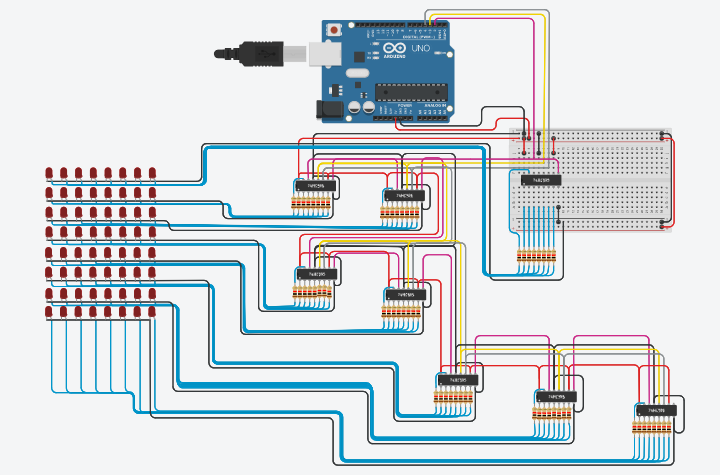
\includegraphics[scale=0.7]{circuito.PNG}
\graphicspath{ {images/} }
\centering
\caption{Circuito de la matriz con leds}
\label{fig:circuito.PNG}
\end{figure}

Las secciones (\ref{intro}), (\ref{contenido}) y (\ref{images}) dependen del estilo del documento.

\bibliographystyle{IEEEtran}


\end{document}
